\documentclass[11pt, twocolumn]{article}  % for review and submission
%\documentclass[aps,preprint,showpacs,superscriptaddress,groupedaddress]{revtex4}  % for double-spaced preprint
\usepackage{graphicx}  % needed for figures
\usepackage{dcolumn}   % needed for some tables
\usepackage{bm}        % for math
\usepackage{amssymb}   % for math
\usepackage{hyperref}  %to use \autoref to reference objects
\usepackage[export]{adjustbox} %alignment of figures

%\linespread{1.8} %double-spacing

\usepackage[hmarginratio=1:1,top=15mm, bottom=15mm, left=15mm, right=15mm,columnsep=20pt]{geometry} % Document margins
%\usepackage{anysize}
%\marginsize{20mm}{20mm}{15mm}{15mm}
%\marginsize{left}{right}{top}{bottom}
%\usepackage[left = 15mm, top = 15mm]{geometry} %margins

\providecommand{\e}[1]{\ensuremath{\times 10^{#1}}} %for scientific notation
\providecommand{\squiggle}{\raise.17ex\hbox{$\scriptstyle\sim$}} %for tilde character

\providecommand{\noNe}[1]{{${#1}\times 10^{19}$ cm$^{-3}$}} % for writing density as a number followed by cm^-3

\providecommand{\neupstream}{$n_{e~upstream}$} % upstream electron density shortcut
\providecommand{\neus}{$n_{e~us}$} % upstream electron density shortcut
\providecommand{\netarget}{$n_{e~target}$} % target electron density shortcut
\providecommand{\netg}{$n_{e~tg}$} % target electron density shortcut
\providecommand{\Tus}{$T_{tg}$} % Upstream temperature shortcut
\providecommand{\Ttg}{$T_{tg}$} % Target temperature shortcut

%\usepackage[left = 15mm, top = 15mm]{geometry} %margins
\usepackage{amssymb} % Allows use of \therefore command to get the three dots in a triangle symbol

%Figures
\usepackage{graphicx}
%syntax:
%\includegraphics[scale=1.0]{filepath.extension}

%bibliog
\usepackage[UKenglish]{babel}
\usepackage{url}
\usepackage[backend=bibtex, style=numeric-comp, sorting=none, doi=false,isbn=false,url=false]{biblatex}
\bibliography{BIBfiles/initial}
% bun citep amirite!!!
\newcommand{\citep}[1]{\cite{#1}}
%stop paper titles being printed in bibliography
\AtEveryBibitem{\clearfield{title}}
%stop "In:" being printed before journal name
\renewbibmacro{in:}{}
%small bibliography font size
\renewcommand*{\bibfont}{\small}

% Appendix
\usepackage[toc,page]{appendix}
%euro symbol (\EUR i think)
\usepackage{eurosym}

% for multirow command in table generation
\usepackage{multirow}

% Document
\begin{document}

\title{Divertor detachment stability and dynamics}
\author{Joe Allen, JOA509}
%\date{\today}

\twocolumn[
\begin{@twocolumnfalse}
    \maketitle
    \begin{abstract}
\noindent Do I need an abstract? Well, if I do then it will go here, spread over both columns. 
	\end{abstract}
\end{@twocolumnfalse}
]

%\tableofcontents

\section{Introduction}\label{sec:Intro}

\section{Background}\label{sec:Bg}
Brief overview of the importance of detachment for ITER and future tokamaks.
- Current material limit
- Divertor geometries (conventional, super-X, snowflake)
- 


\section{Experimental Design}\label{sec:Expt}
SOL1D was installed on the remote server and some test simulations run to achieve a basic understanding of the set-up and outputs. The first aim was to ascertain an acceptable grid resolution to use, as a compromise is required concerning accuracy of results and time taken to run a simulation. SOL1D performs 1-dimensional simulations and the y-axis was chosen as the simulation axis. 

Following SOL1D simulations, 2D simulations follow, with the initial goal being to compare results to the 1D case.

\section{Results and Analysis}\label{sec:Results}
\subsection{SOL1D}\label{ssec:SOL1D}
After a number of time-steps of SOL1D simulation it will usually settle down and get close to a steady-state solution. This can be seen in figure~\ref{fig:ne_var_ny=800} - the variable's, \neupstream, oscillations are damped to a very small amplitude as the simulation progresses and it approaches steady-state, which took about 24 hours to reach its current point. Perhaps the simulation could have been stopped earlier, however this would increase the uncertainty in all the output data. Simulations with lower resolution do not reach a steady state in fewer time points, but they are faster to run so they reach it quicker in real time.

\begin{figure}
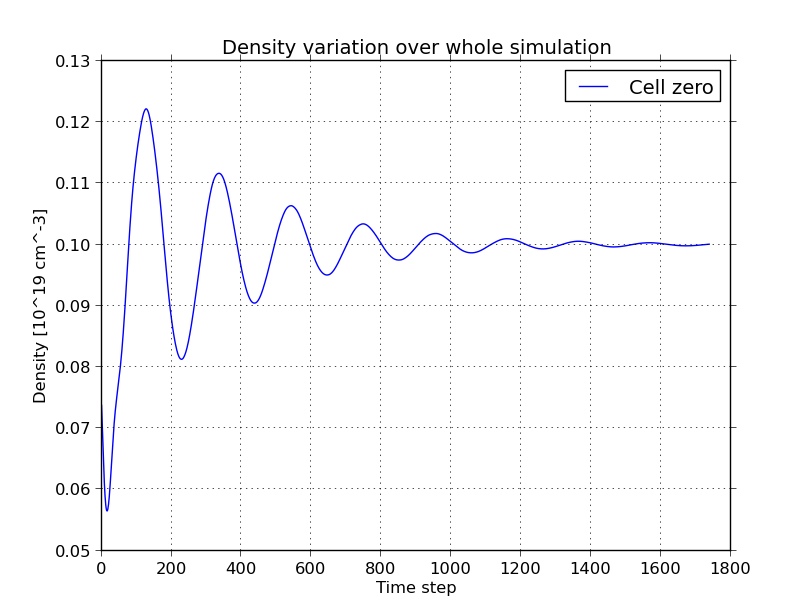
\includegraphics[scale=0.4]{Figures/sol1d/ne_var_ny=800.png}
\centering
\caption{The variation of \neus with simulation time step. \textbf{should maybe put the oscillations from other resolutions on the same figure to make it more interesting?}}\label{fig:ne_var_ny=800}
\end{figure}

An important first step when running grid simulations is to ascertain an acceptable resolution to use. Figure~\ref{fig:RichExtrp_neres} shows the approximate steady-state value of \netarget for different resolutions. The choice of resolution has to take into account the accuracy of the output and the time taken to receive said output. It is clear that \netg is tending towards a value at infinite resolution. There is a 5.0\% change from 200 to 400 cells, 1.6\% change from 400 to 600 and 0.58\% change from 600 to 800 cells. Given that the number of operations performed by the code scales as approximately $N^2$ for $N$ cells, increasing the cell number heavily increases the computing cost. Table~\ref{tab:sol1dres} contains run times at different resolutions, and shows a stark increase in time for increasing resolution. The second run, at \neus $= 1.25\e{19}$ cm$^{-3}$, completed significantly faster than the first run because it was restarted from the near steady-state snapshot at the end of the first run. Therefore, each simulation time step is completed faster because the system is already rather stable, and only needs to accommodate an injection of an extra $0.25\e{19}$ cm$^{-3}$ of material in from the upstream.

\begin{table}[]
%\centering
\caption{SOL1D simulation run times with different resolutions.}
\label{tab:sol1dres}
\begin{tabular}{l|l|l|l}
\multicolumn{1}{l|}{\multirow{2}{*}{}} & \multicolumn{3}{l}{Time taken to complete 1000 time steps}    \\ \cline{2-4} 
 \multicolumn{1}{l|}{Resolution}        & \multicolumn{1}{l|}{\neus: $1.0\e{19}$ cm$^{-3}$} & \multicolumn{1}{l|}{$1.25\e{19}$ cm$^{-3}$}  &  \\ \hline
                   200                 &      47m 44s          &    24m 23s         &  \\
                   400                 &      1h 48m 55s       &    2h 45m 4s       &  \\
                   600                 &      7h 40m 57s       &    5h 5m 4s        &  \\
                   800                 &      13h 18m 55s      &    7h 1m 28s       &  
\end{tabular}
\end{table}

\begin{figure}
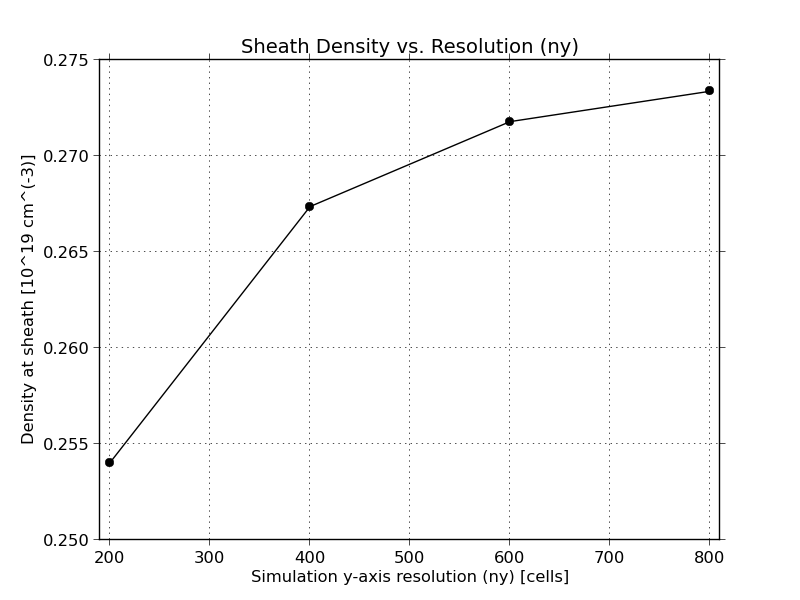
\includegraphics[scale=0.4]{Figures/sol1d/RichExtrp_neres.png}
\centering
\caption{Density at sheath, \netg, at approximately steady-state for different y-axis resolutions in SOL1D.}\label{fig:RichExtrp_neres}
\end{figure}

\subsubsection{Temperature comparison}\label{sssec:tempcomp}
Two key parameters to be analysed are the upstream and target temperatures, \Tus and \Ttg. The whole point of divertor detachment is to reduce the power flux impacting on the divertor. \Ttg sets the voltage across the sheath, which in turn influences the velocity of ions impacting on the solid divertor target (ions in the simulation have a fixed velocity when entering the sheath - the Bohm velocity). The lower \Ttg, the less damage will be done to the divertor plates. Figure~\ref{fig:TT_IMPCOMBO2} shows the difference between \Tus and \Ttg for different \neus values at each of the resolutions in table~\ref{tab:sol1dres}. When looking to reduce \Ttg, the trade off is the corresponding fall in \Tus. As the upstream is at the SOL midplane, any changes there will be translated directly into the main plasma. 

Similarly shaped temperature profiles are observed for all resolutions in figure~\ref{fig:TT_IMPCOMBO2}, \Tus falls slowly while \Ttg falls rapidly with increasing \neus, until above $2.25\e{19}$ cm$^{-3}$ when it starts to fall extremely fast. At this point, the density profile has pulled away from the divertor and this extra density flooding into the upstream is reducing the temperature there. If an operational 'sweet-spot' exists, then it is in the range $2\e{19}$ cm$^{-3}$ < \neus < $2.25\e{19}$ cm$^{-3}$, as here \Ttg has practically reached it's lower limit while \Tus is still quite high.

\begin{figure}
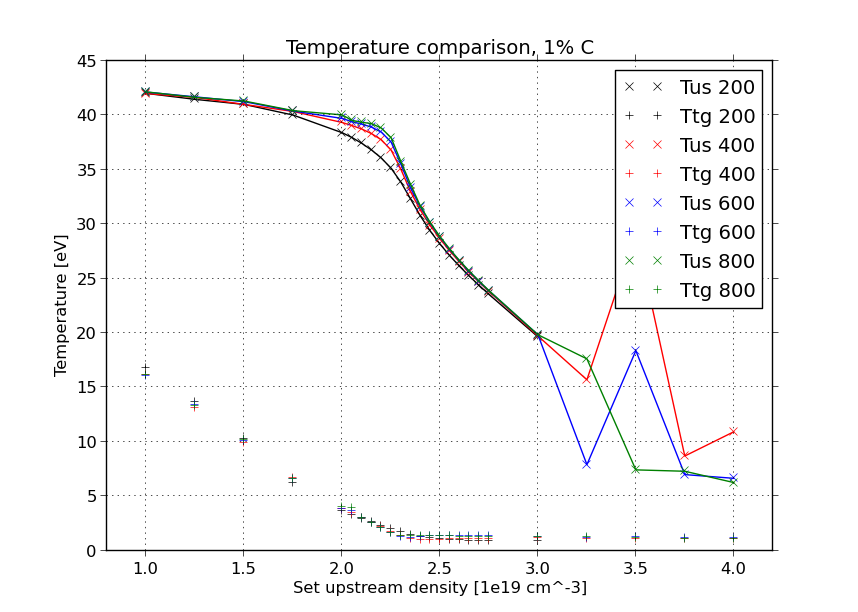
\includegraphics[scale=0.5]{Figures/sol1d/TT_IMPCOMBO2.png}
\centering
\caption{Comparison of $T_{upstream}$ and $T_{target}$ at varying set $n_{e~upstream}$ for different y-axis resolutions in SOL1D}\label{fig:TT_IMPCOMBO2}
\end{figure}

Simulations from \noNe{3} onwards shown in figure~\ref{fig:TT_IMPCOMBO2} are detaching and reattaching in quick succession, so they are unlikely to approach a steady state within a reasonable number of timesteps. When detached, the upstream temperatures in these simulations follow the downward trend observed with increasing \neus. However, when the system destabilises and rushes to reattach to the target plates, the upstream temperature shoots up. If these higher density simulations are terminated during a period of detachment, \Tus will be low, as is the case for all the \noNe{3.75} runs. Conversely, if they are terminated when the density profile has reattached, \Tus will be much higher, which can be seen in the data points at \noNe{3.5} for ny = 400 \& 600 cells. This cyclical detachment and reattachment is portrayed in figure~\ref{fig:ny400800r35netg} - here \netg is observed following a pattern of peaks (when system is attached to the target) and troughs (when the system is detached). In the case of the black line, with y-axis resolution of 400 cells, the simulation has completed when the sheath density is still far higher than its minimum value, so the density profile is still in the process of detaching from the target surface. Consequently, the upstream temperature is still relatively quite high. The red line is from a simulation with the same input values but using 800 cells along the y-axis, here termination has occurred when the density profile is almost fully detached from the target, hence the upstream temperature is quite low. This termination snapshot effect can be seen in figure~\ref{fig:TT_IMPCOMBO2} at \noNe{3.5}, where the upstream temperature with 400 cells is much higher than that for 800 cells.

\begin{figure}
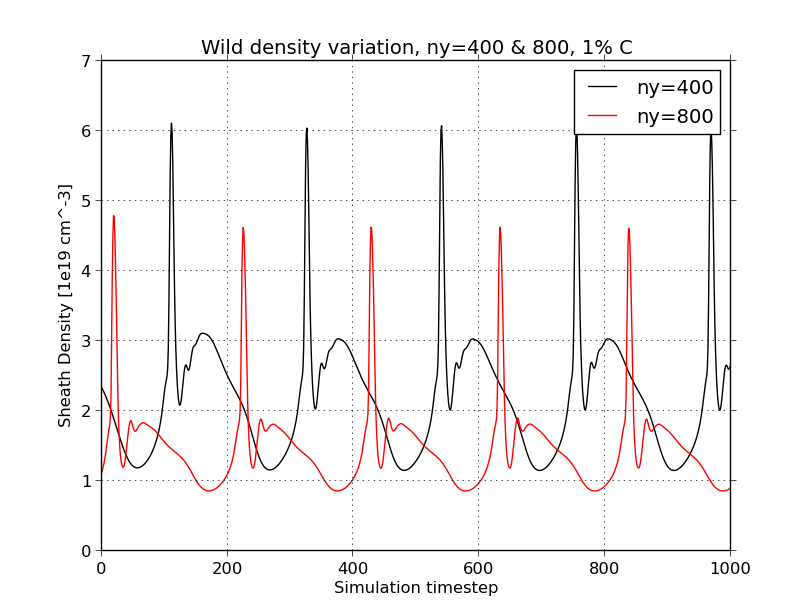
\includegraphics[scale=0.5]{Figures/sol1d/ny400800r35netg.png}
\centering
\caption{Continual detachment and reattachment causes the target $n_e$ variations for ny = 400 and 800 cells run with \neus~set to \noNe{3.5}.}\label{fig:ny400800r35netg}
\end{figure}


\subsubsection{Pressure Loss}\label{sssec:Ploss}

Experimentally, pressure loss ratio saturates at high target temperatures due to the relation between static and viscous (?) pressure (maths is on p18 of lab book) and falls sharply as 

\begin{figure}
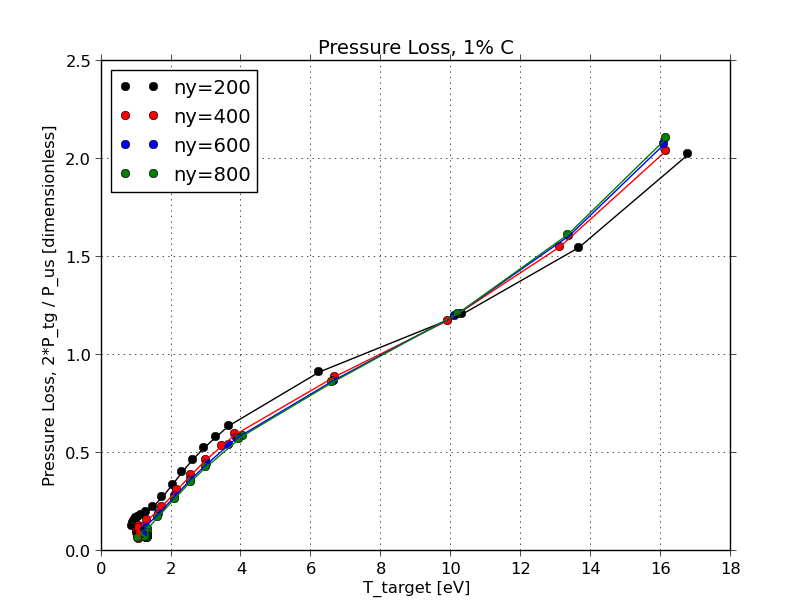
\includegraphics[scale=0.5]{Figures/sol1d/PL_IMPCOMBO2.png}
\centering
\caption{Pressure loss ratio, $\frac{2P_{tg}}{P_{us}}$, change with \Ttg at different y-axis resolutions in SOL1D.}\label{fig:PL_IMPCOMBO2}
\end{figure}

\begin{figure}
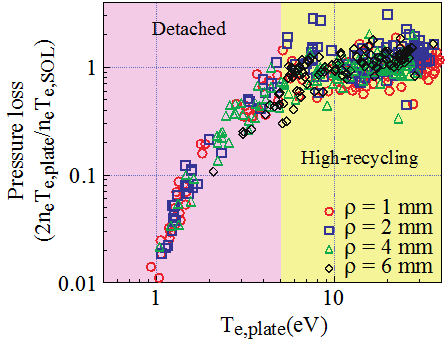
\includegraphics[scale=1]{Figures/PlossAlcator.png}
\centering
\caption{Pressure loss ratio, $\frac{2P_{tg}}{P_{us}}$, data from Alcator C-Mod \cite{Lipschultz2007}.}\label{fig:PlossAlcator}
\end{figure}


\section{Conclusion}\label{sec:Conclusion}




\printbibliography

\end{document}
